\documentclass[12pt]{article}

\usepackage[utf8]{inputenc}
\usepackage[french]{babel}
\usepackage{lmodern}	
\usepackage[top=3cm, bottom=3cm, left=3cm, right=3cm]{geometry}
\usepackage{graphicx}
\usepackage{array}
\usepackage[T1]{fontenc}
\usepackage{xcolor}
\usepackage{listings}
\usepackage{float}
\usepackage{listings}
\usepackage{pgf}
\usepackage{tikz}
\usetikzlibrary{arrows,automata}
\usepackage{verbatim}
\usepackage{algorithmic}

\floatplacement{figure}{H}
\newcommand{\HRule}{\rule{\linewidth}{0.5mm}}
%PYTHON
\DeclareFixedFont{\ttb}{T1}{txtt}{bx}{n}{10} % for bold
\DeclareFixedFont{\ttm}{T1}{txtt}{m}{n}{10}  % for normal

% Custom colors
\usepackage{color}
\definecolor{deepblue}{rgb}{0,0,0.5}
\definecolor{deepred}{rgb}{0.6,0,0}
\definecolor{deepgreen}{rgb}{0,0.5,0}

\usepackage{listings}

% Python style for highlighting
\newcommand\pythonstyle{\lstset{
language=Python,
basicstyle=\ttm,
otherkeywords={self},             % Add keywords here
keywordstyle=\ttb\color{deepblue},
emph={MyClass,__init__},          % Custom highlighting
emphstyle=\ttb\color{deepred},    % Custom highlighting style
stringstyle=\color{deepgreen},
frame=tb,                         % Any extra options here
showstringspaces=false            % 
}}


% Python environment
\lstnewenvironment{python}[1][]
{
\pythonstyle
\lstset{#1}
}
{}

% Python for external files
\newcommand\pythonexternal[2][]{{
\pythonstyle
\lstinputlisting[#1]{#2}}}

% Python for inline
\newcommand\pythoninline[1]{{\pythonstyle\lstinline!#1!}}
%END_PYTHON
\begin{document}
\begin{titlepage}
  \begin{center}
    \textsc{\LARGE Université Pierre et Marie Curie}\\[1.5cm]
    
\includegraphics[height=1cm]{upmc.png}\\[1.5cm]
    \textsc{\Large Rapport VLSI 2 }\\[2cm]

    \HRule \\[1cm]
    \textsc{\huge Rapport TP's VLSI 1 \& 2 \& 3 }\\[0.5cm]
    \HRule \\[1cm]

    % Author and supervisor
    \noindent
    \begin{minipage}[t]{0.55\textwidth}
      \begin{flushleft} \large
        \emph{Auteurs:}\\
        BITAM \textsc{Massine}\\
        BRAND \textsc{Andres}
      \end{flushleft}
    \end{minipage}%
    \begin{minipage}[t]{0.47\textwidth}
      \begin{flushright} \large
        \emph{Encadrant:} \\
        Wajsburt \textsc{Franck}
      \end{flushright}
    \end{minipage}

    \vfill

    % Bottom of the page
    {\large \today}
  \end{center}
  \newpage
  \tableofcontents
  \newpage
  \listoffigures
  \newpage
\end{titlepage}
\section{Remarque}
Les fichiers sont dans les répertoires nommés lab1, 2, 3, et toutes les étapes sont automatisées avec un makefile.\\
Les fichiers sont aussi disponible sur github : https://github.com/Masshat/VLSI/
\section{TP1: Synthèse Logique}
\subsection{Introduction}
Le but de ce TP est l'étude de la partie front-end du flot de conception VLSI qui est la description comportementale d'un circuit numérique en VHDL (res:verilog) à partir d'une spécification papier (datasheet) en vue d'arriver à obtenir une netlist de portes. 
Ceci est l'étape de synthèse.\\
Connaissant déjà le flot de conception d'un circuit numérique VLSI et ayant déjà eu auparavant une première expérience avec les outils alliance que nous avons utilisé dans UE: VLSI 1 où nous avons réalisé un processeur (AM2901), à partir de sa datasheet jusqu'à l'obtention du layout final, ainsi que l'analyse de timing, nous avons décidé d'aller jusqu'au bout de ce TP en utilisant les mêmes outils, mais cette fois si, grâce au cours où on  nous a détaillé et  expliqué l'utilisation et le réglage des outils afin d'optimiser certaines parties du flot et ainsi, obtenir à la fin de chaque étape des vues correctes et un circuit optimisé.\\

\subsection{Synthèse}
Dans ce TP nous avons utilisé un style particulier de description VHDL qui est la description d'un circuit sous forme de machine à état (FSM). Après s'être familiarisé avec ce style de description via l'exemple du compteur, nous avons réalisé un digicode en suivant les instructions données. Nous avons commencé donc par écrire le code VHDL de notre automate, préalablement modélisé à la main.\\

Avant d'entamer l'étape de synthèse, nous avons utilisé l'outil \textbf{xfsm} afin de visualiser les états et les transitions entre ces derniers et ainsi valider notre automate. Le fichier de description d'un fsm avec les outils alliance porte l'extension .fsm .\\
\begin{figure}
\begin{center}
  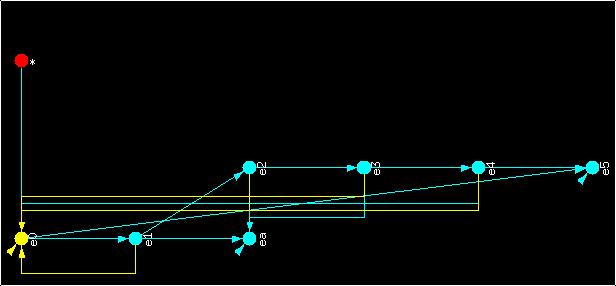
\includegraphics[width = 11cm]{pic/fsm.png}
\end{center}
\caption{représentation de fsm du digicode.}
%\label{fig 1.}
\end{figure}

 L’outil syf permet ainsi de générer une description comportementale à partir de la description fsm avec cette fois si l'extension .VHDL. C'est cette dernière qui sera synthétisé.\\

Apres avoir généré une description comportementale de notre design, il est important de la simuler pour s'assurer qu'elle implémente bien la fonctionnalité voulue. Pour cela nous procédons à l'étape de simulation avec l'outil \textbf{ASIMUT}. asimut permet de simuler deux types de description VHDL : comportementale ou structurelle. Nous devons donner ensuite à asimut un fichier avec l'extension .pat en entrée qui comporte les stimuli que l'on va fournir sur les entrées du circuit, et éventuellement les valeurs de sorties attendues ; la première partie consiste à appeler asimut avec l'option -b pour lui indiquer que l'on simule une description comportementale, et -c pour indiquer à asimut de compiler le design, vérifier si un fichier a été donné en entrée pour qu'il soit compilé et linké à la description HDL. Apres cela nous pouvons simuler notre description toujours avec asimut qui va  écrire les résultats de la simulation dans un fichier output.pa. Ce dernier sera lu et interprété par xpat afin de pouvoir visualiser les waveform de la simulation avec l'outil xpat.\\

\begin{figure}
\begin{center}
  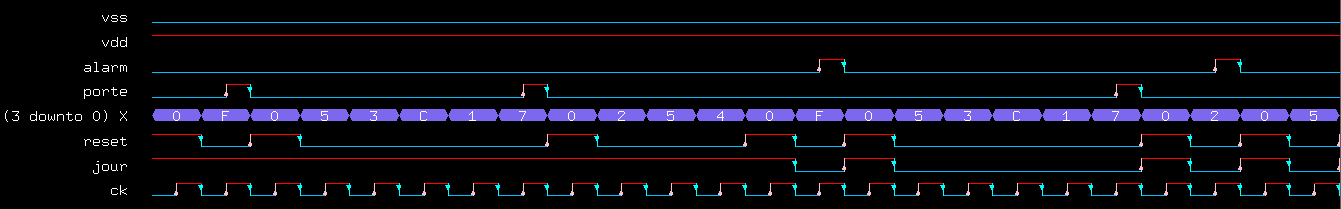
\includegraphics[width = 16cm]{pic/asimut.png}
\end{center}
\caption{résultat de la  simulation.}
%\label{fig 1.}
\end{figure}Avant d'entamer l'étape de synthèse nous détaillons et expliquons les options de l'outil \textbf{Syf}:\\
\begin{itemize}
\item -C : permet de vérifier la consistance des transitions autrement dit: les propriétés de  complétude  et d'orthogonalité de fsm.
\item -E : sauvgarde l'encodage dans un fichier output.enc, ce fichier a la même syntaxe que le fichier input.enc quand on utilise l'option -u afin de définir un encodage personnalisé.
\item -V : mode verbose.
\item -\{a,j,o,m,u,r\} est l'encodage utilisé, nous avons utilisé l'option -o pour onehot.
\end{itemize}
Une fois la description comportementale obtenue nous pouvons passer à l'étape de synthèse qui se décompose en trois sous étapes:
\begin{enumerate}
\item La première étape de synthèse est l'optimisation des équations booléennes, l'outil \textbf{BOOM} permet de faire cela à partir d'une description comportementale en utilisant une représentation RBDD \textbf{\{Reduced Ordered Binary Decision Diagram\}} des fonctions logiques.\\
Nous avons choisi le niveau d'optimisation le plus élevé avec l'option -l et une optimisation maximale en surface avec l'option -d=0. Nous pensons que pour un digicode, il est plus important d'optimiser la surface et ainsi réduire le cout de conception que de jouer sur la fréquence qui n'est pas très importante pour ce genre de circuit.\\
Cette première étape permet d'avoir une description toujours comportementale mais optimisée.
\item La seconde étape de synthèse consiste à réaliser la projection structurelle du comportement sur la bibliothèque de cellules \textbf{Sxlib} afin d'obtenir la netlist. En d'autres termes, plus techniques, l'outil \textbf{BOOG} map \{ Désolé pour l'anglicisme\}, la description comportementale sur la standard cell library afin de générer une description structurelle. L'outil commence par construire le réseau booléen équivalent à la description obtenue avec \textbf{BOOM} puis pour chaque fonction booléenne  de chaque nœud du réseau, il tente de trouver une cellule ou un ensemble de cellules  qui implémentent cette fonction. Le résultat sera une description structurelle basée sur les cellules pré caractérisées. \textbf{SxLib}. Nous obtenons un fichier de la description structurelle (la netlist) au format .vst .
Avant d'aller plus loin nous avons pris la peine de voir le contenu du fichier vbe généré avec BOOM, le code est quasi incompréhensible car il a été optimisé. Nous avons remarqué deux points très importants:
\begin{enumerate}
\item L'outil a rajouté : \color{red}signal \color{black}circuit\_cs : \color{red}REG\_VECTOR\color{green}(6 DOWNTO 0) \color{black}REGISTER, ce signal sera intérprété par Boog comme le registre d'états de l'automate.
\item \color{red}signal \color{black}circuit\_ef : \color{red}BIT\_VECTOR\color{green}(6 DOWNTO 0)\color{black}; qui représente la valeur de chaque bascule constituant l'état futur que prendra l'FSM au prochain front montant d'horloge.
\end{enumerate}
Après cela, l'outil boug comme nous l'avons expliqué plus haut, va associer à chaque bit du registre d'états une structure sff\_x qui représente une bascule. Ceci est visible dans la netlist vue avec xsch.
\item La dernière étape de synthèse est l'optimisation électrique avec l'outil \textbf{LOON}.\\
Les options utilisées avec Loon sont -x afin de générer une netlist colorée des chemins critiques, et l'option -m 0 afin d'optimiser la surface.\\
Afin de visualiser la netlist nous utilisons l'outil xsch qui permet aussi de chercher le nom d'une cellule ou d'un signal particulier.

\begin{figure}
\begin{center}
  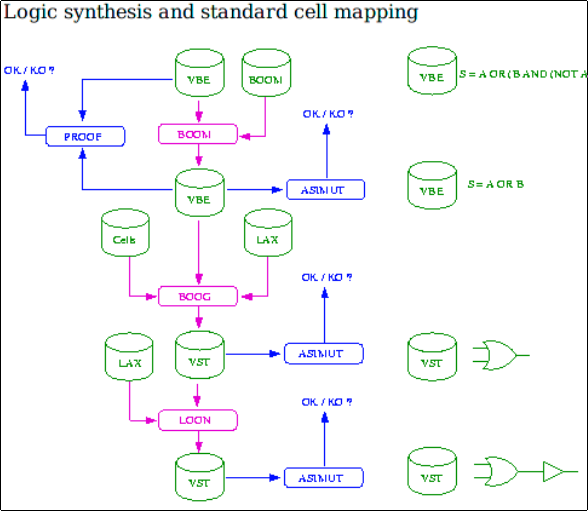
\includegraphics[width = 8cm]{pic/process.png}
\end{center}
\caption{Les étapes de la synthèse.}
%\label{fig 2.}
\end{figure}

\end{enumerate}
Dans cette figure, nous pouvons observer que le signal d'horloge attaque bien toutes les bascules qui représentent le registre d'états de FSM.
\begin{figure}
\begin{center}
  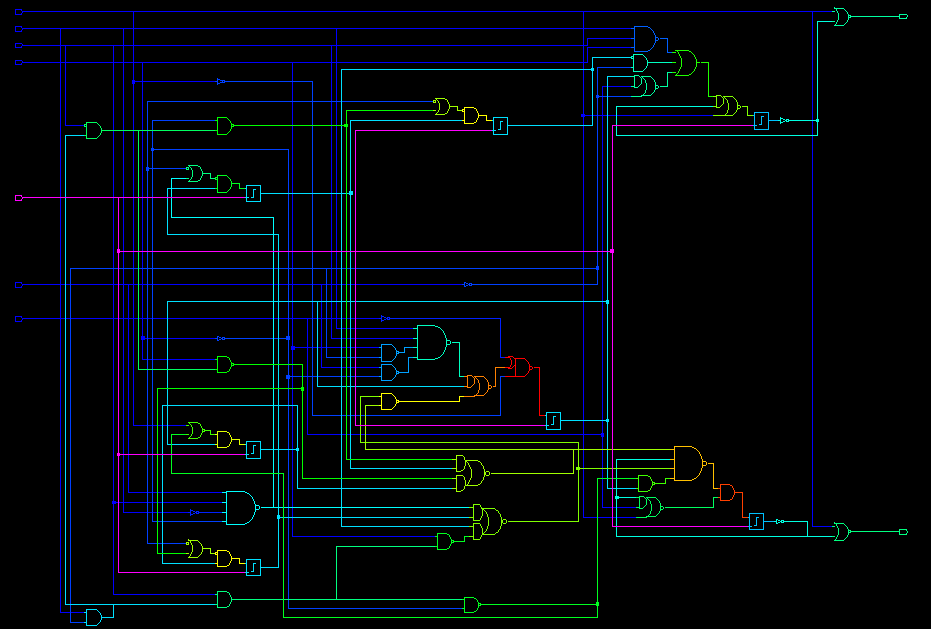
\includegraphics[width = 12cm]{pic/clk.png}
\end{center}
\caption{Le signal d'horloge.}
%\label{fig 2.}
\end{figure}

Dans cette figure nous pouvons observer que le signal reset attaque bien des bascules qui représentent le registre d'états de FSM afin de le réinitialiser à l'état IDLE et aussi les sorties du circuit pour sortir les bonnes valeurs en cas de reset.
\begin{figure}
\begin{center}
  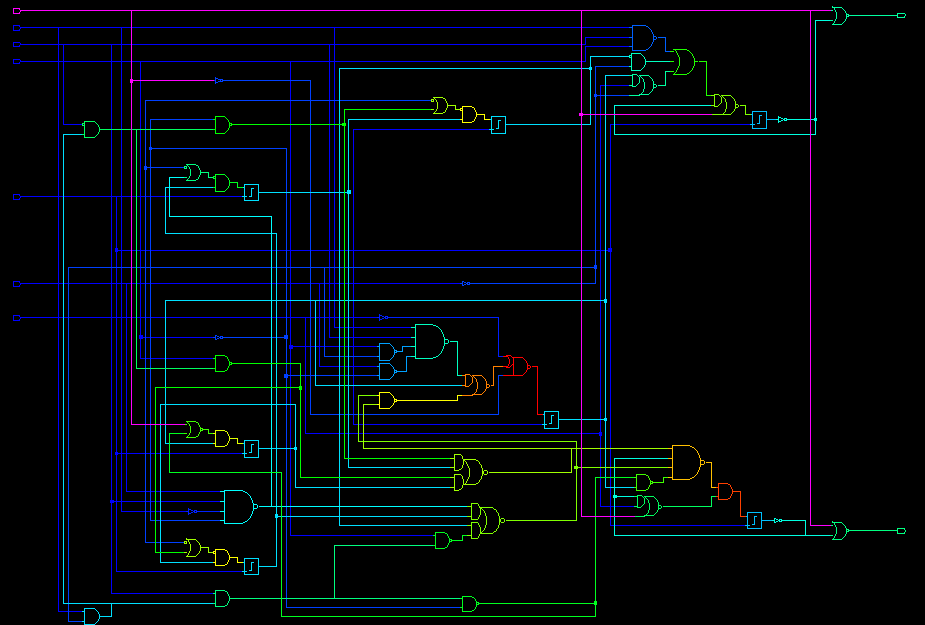
\includegraphics[width = 12cm]{pic/reset.png}
\end{center}
\caption{Le signal reset.}
%\label{fig 3.}
\end{figure}

Dans cette figure nous pouvons observer le chemin critique de notre circuit avec le timing arc de notre cellule.

\begin{figure}
\begin{center}
  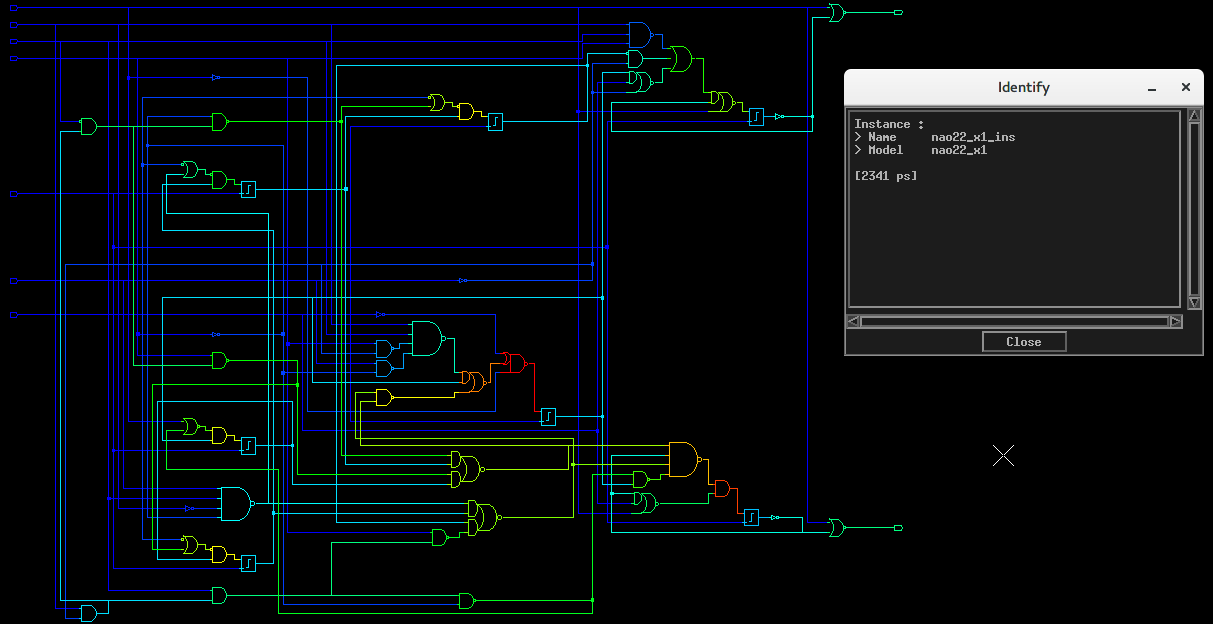
\includegraphics[width = 12cm]{pic/critical.png}
\end{center}
\caption{Le chemin critique.}
%\label{fig 4.}
\end{figure}

ubsection{Verification formelle des deux netlist}
Avant de passer à l'étape de placement routage, il est important de vérifier que l'étape de synthèse s'est bien passé, ainsi nous devons extraire la description comportementale à partir de la netlist obtenue, et la comparer avec la première décrite ou générée grâce à syf. Il faut que les deux descriptions soit identiques, elles doivent assurer la même fonctionnalité.\\
Pour vérifier cela, nous utilisons un outil de vérification formel \textbf{proof} qui compare ainsi deux descriptions comportementales.\\
Afin d'extraire la description comportementale de la structurelle nous utilisons l'outil Flatbeh, après cela nous pouvons appeler  proof et ainsi valider notre netlist.

\subsection{Placement \& Routage}
Les étapes décrites précédemment sont ce que l'ont appelle la partie front-end en conception d'ASIC. A partir de là, nous nous situons sur la partie back-end qui est le P \& R, la vérification des règles de dessin DRC \{{Design Rules Cheking}\}, la vérification LVS \{{Layout versus sémantic}\} et le passage d'un layout en représentation symbolique au layout réel.

L’étape qui suit la synthèse, est le placement/routage. Nous utilisons les deux outils ocp pour le placement et néro pour le routage.\\
L'outil OCP permet de faire le placement. Nous lui fournissons en entrée un fichier .ioc pour lui indiquer le placement des pins d'entrées/sorties du circuit.\\Voici le résultat du placement:

\begin{figure}
\begin{center}
  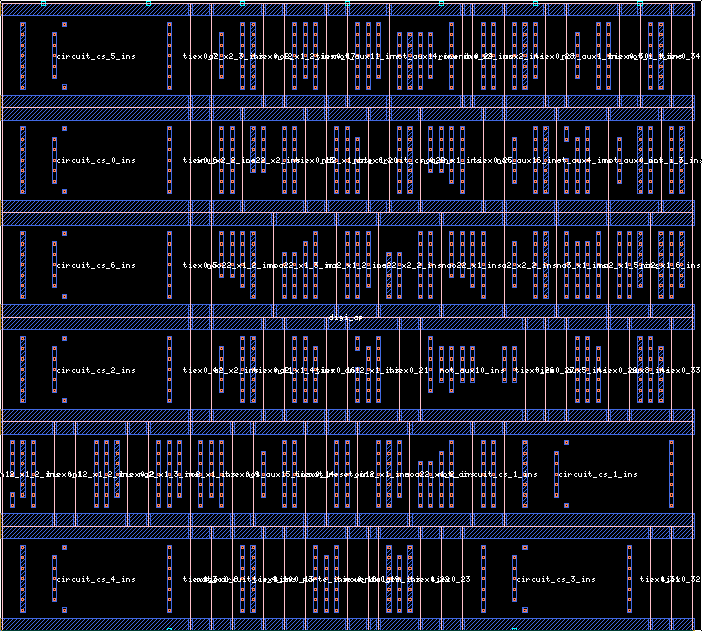
\includegraphics[width = 10cm]{pic/place.png}
\end{center}
%\caption{Le chemin critique.}
%\label{fig 4.}
\end{figure}

L'outil NERO permet de faire le routage du circuit en prenant une netlist déjà placée. Voici le résultat du routage:

\begin{figure}
\begin{center}
  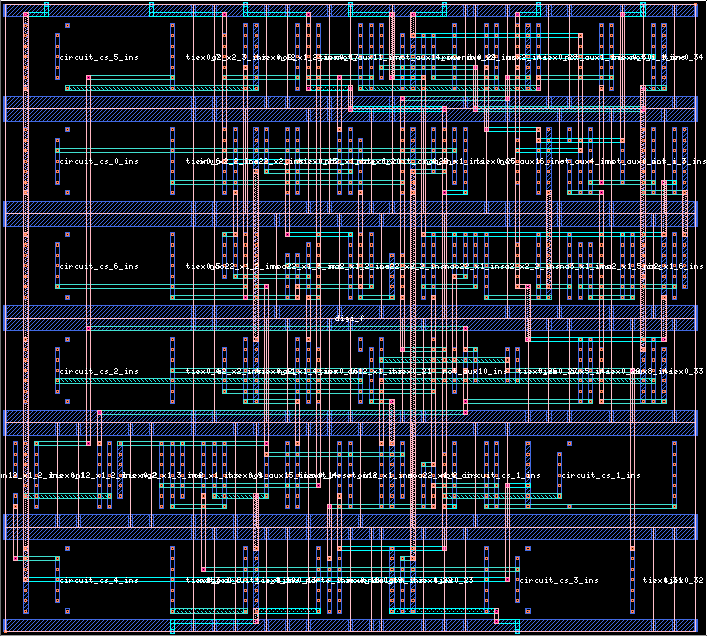
\includegraphics[width = 10cm]{pic/route.png}
\end{center}
\end{figure}

\subsection{Verification du layout}
Une fois le placement routage fini, nous avons enfin obtenu notre layout que nous pouvons visualiser avec graal. L'étape suivante est la vérification du dessin des masques obtenus ; il y'a deux vérifications à faire : la première est la vérification des règles de dessin avec l'outil \textbf{Druc}, la seconde est de vérifier si la netlist extraite avec cougar avec l'option -ac pour enlever toutes les capacités, et de pouvoir faire une analyse de timing plus tard. La vérification se fait ensuite avec lvx  qui  comparera la netlist obtenue après synthèse et celle extraite avec cougar. Cette étape permet de valider si le P \& R s'est bien passé ou pas.
\subsection{Obtention du dessin de masque final}
La dernière étape du flow de conception VLSI, est l'obtention du dessin des masques à envoyer en fonderie. Ce fichier est au format cif ou GDS2. Nous avons utilisé l'outil \textbf{S2R} pour le passer de dessin symbolique à réel.  Nous obtenons finalement le fichier à l'extension cif, qui est notre layout final.
\subsection{Makefile}
Comme nous l'avons précisé au début du rapport, tout a été automatiser par un Makefile:\\
make all: permet de faire la simulation, la synthèse, et le placement routage.\\
make tp: permet d'automatiser tout ce qui a été demandé dans le tp.\\
make check: permet de vérifier l'équivalence de netlist avec cougar et lvx.\\
make druc: permet de vérifier les régles de dessin.\\
make s2r: permet d'obtenir le fichier cif.\\
make proof: permet de vérifier formellement les netlist.\\
make dreal, xsch, xfsm, xpat: permet d'appeler les différents outils de visualisation.\\
Il y'a aussi des variables qui servent à choisir l'encodage utilisé comme ENC, le degré d'optimisation L et le paramètre D qui est le compromis entre la surface et le délai en terme d'optimisation de netlist.\\
\subsection{Réponses des questions posées dans le TP}
\begin{enumerate}
\item Si le reset n'est pas positionné au début du pattern, le système démarrera dans un état inconnu. Nous avons vu avec Mr Tuna, que la gestion de ce signal est critique car très importante. Afin de mettre le circuit dans un état connu, nous avons effectué aussi nos propres recherches et nous avons découvert qu’il y a dans tous les circuits un système appelé POWER\_ON\_RESET qui utilise une bascule de Schmitt afin de reset le circuit au démarrage.

\item selon nous la meilleure netlist est la netlist optimisée en surface comme nous l'avons précisé plus haut.(pour ce genre de circuit bien sur!!)
\end{enumerate}
\newpage
\section{TP2: Stratus / Placement \& Routage}
\subsection{Introduction}
Dans ce TP nous avons décrit des netlist en python avec la suite stratus après avoir suivi les exemples donnés dans le TP. Nous avons pu générer les differents blocs constituant l'addaccu.  Voici les figures de nos composants mux(4bits), full\_adder (1 bit), adder (4 bits)  et accu (4 bits). Nous avons pu décrire et valider ces derniers sans trop de problèmes. Les schémas de netlist sont:

\begin{figure}
\begin{center}
  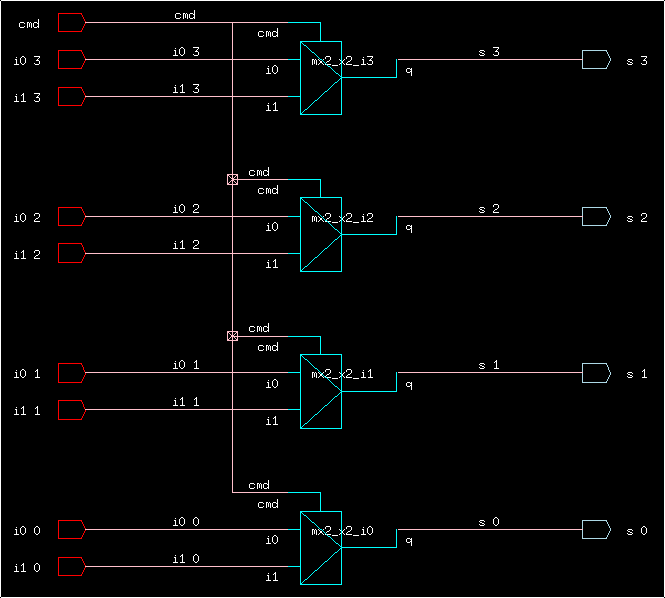
\includegraphics[width = 7cm]{pic/mux.png}
\end{center}
\caption{Bloc Mux.}
%\label{fig 4.}
\end{figure}
 
\begin{figure}
\begin{center}
  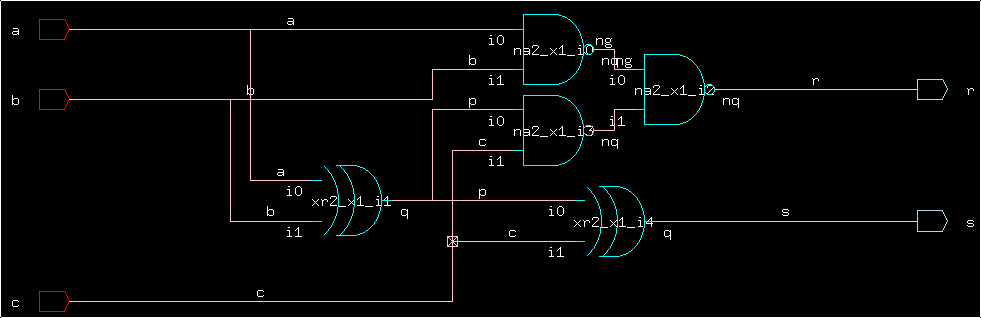
\includegraphics[width = 9cm]{pic/fa.png}
\end{center}
\caption{Full\_adder.}
%\label{fig 4.}
\end{figure}

\begin{figure}
\begin{center}
  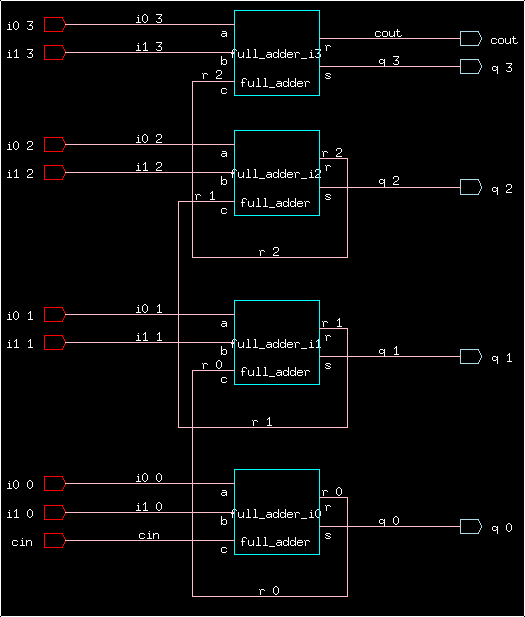
\includegraphics[width = 7cm]{pic/adder.png}
\end{center}
\caption{Bloc Adder.}
%\label{fig 4.}
\end{figure}

Pour l'accumulateur nous avons choisi d'implémenter des flip-flop statiques même si celles ci prennent plus de surface comparées aux flip-flop dynamiques. Nous avons quand même choisis ces dernières pour deux raisons:
\begin{enumerate}
\item notre circuit est quasi combinatoire et l'accumulateur est la seule partie séquentielle, nous pouvons donc nous permettre d'implémenter des bascules statiques.
\item avec ce genre de bascules nous pouvons utiliser la technique de clock\_gating qui permet de réduire la consommation en coupant l'horloge aux bascules  sans perdre la valeur qu'elles contiennent.
\item un dernier avantage est que, si notre signal d'horloge peut être instable ou scrétché à certains moments, nous sommes sûrs que la valeur mémorisée ne sera pas perdue! 
\end{enumerate}

\begin{figure}
\begin{center}
  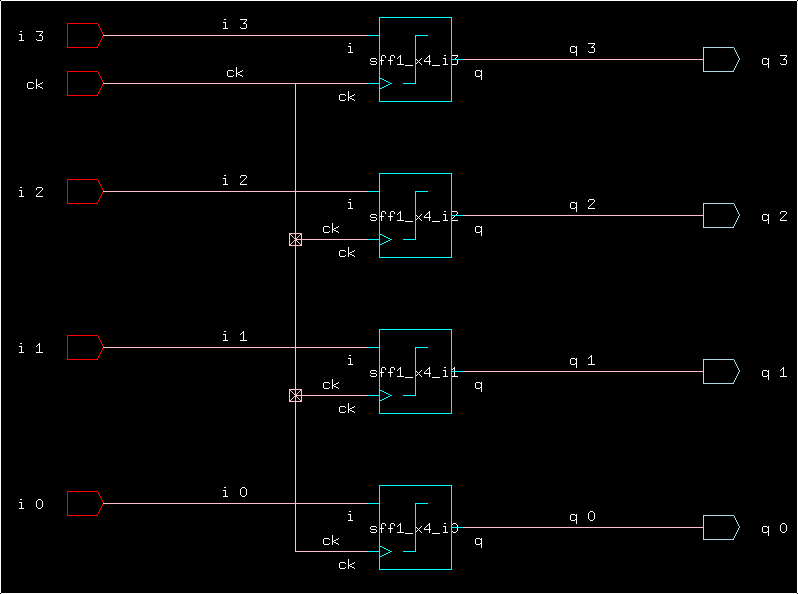
\includegraphics[width = 7cm]{pic/accu.png}
\end{center}
\caption{Bloc Accu.}
%\label{fig 4.}
\end{figure}
La difficulté rencontrée dans ce TP est que lors de l'assemblage des composants pour créer l'addaccu, nous avons oublié que l'ont ne pouvait pas affecter un signal sur une sortie et en même temps le réutiliser (le lire) par une autre entité dans le design ; ce qui explique le rajout des composants buffer en VHDL. Il faut ou créer un signal intermédiaire qui se traduira par des buffers en synthèse ou  déclarer le port de sortie en tant que \textbf{buffer} et non en \textbf{out}.
Voici la netlist finale de notre circuit addaccu:
\begin{figure}
\begin{center}
  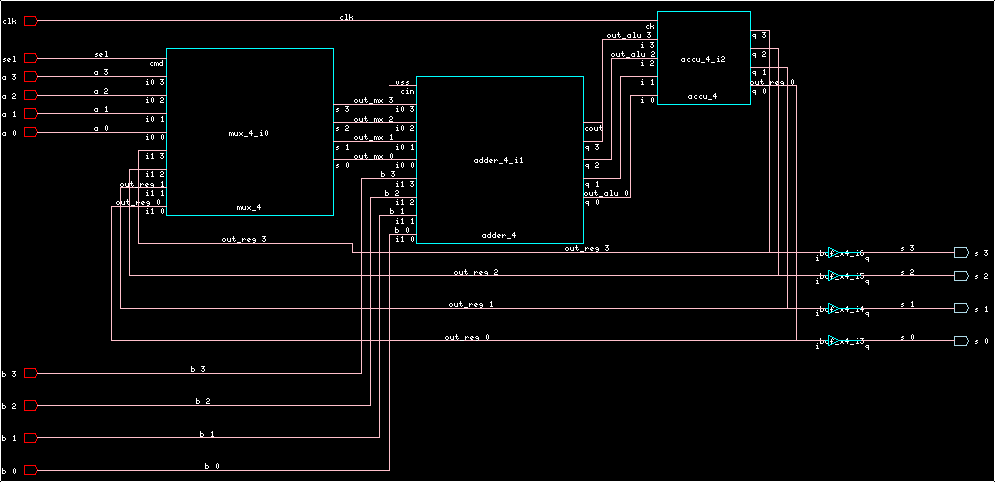
\includegraphics[width = 12cm]{pic/addaccu.png}
\end{center}
\caption{Netlist Addaccu.}
%\label{fig 4.}
\end{figure}
Afin de générer la netlist de l'addaccu, nous avons introduit les deux mécanismes de génération dans le makefile:\\
make : permet de générer l'addaccu avec la fonction generate.\\
make dpgen : permet de générer l'addaccu avec avec \textbf{dpgen}.\\
Au tout début du makefile vous pouvez définir le nombre de bits grâce au paramètre N.\\

\subsection{générateur utilisé}
\begin{tabular}{|l|l|l|}
\hline 
Composant & Générateur & Description \\
\hline
mux    &  DpgenMux2   &  Generates a n bits two inputs multiplexer with an output\\ 
       &	      &  power of d named modelname.\\ \hline
adder  &  DpgenAdsb2f &  Generates a n bits adder/substractor named modelname.\\ \hline
accu   &  DpgenSff    &  Generates a n bits static flip-flop named modelname.\\ \hline
buffer &  DpgenBuff   &  Generates a n bits inverter with an output power of d\\
       &              &   named modelname.\\
\hline
\end{tabular}
\subsection {L'outil CGT}
Une fois notre netlist obtenue, nous avons procédé au placement routage avec l'outil \textbf{CGT}, voici les différents layouts obtenus.
\begin{figure}
\begin{center}
  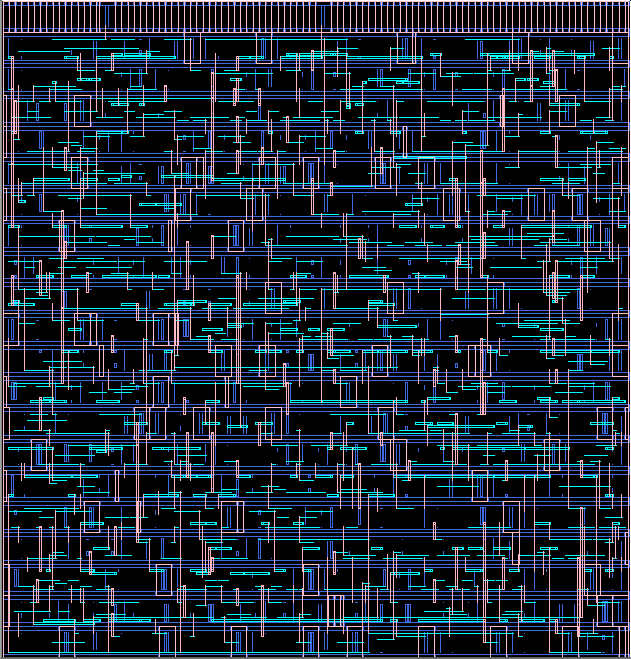
\includegraphics[width = 7cm]{pic/standard.png}
\end{center}
\caption{Circuit glue logique.}
%\label{fig 4.}
\end{figure}

\begin{figure}
\begin{center}
  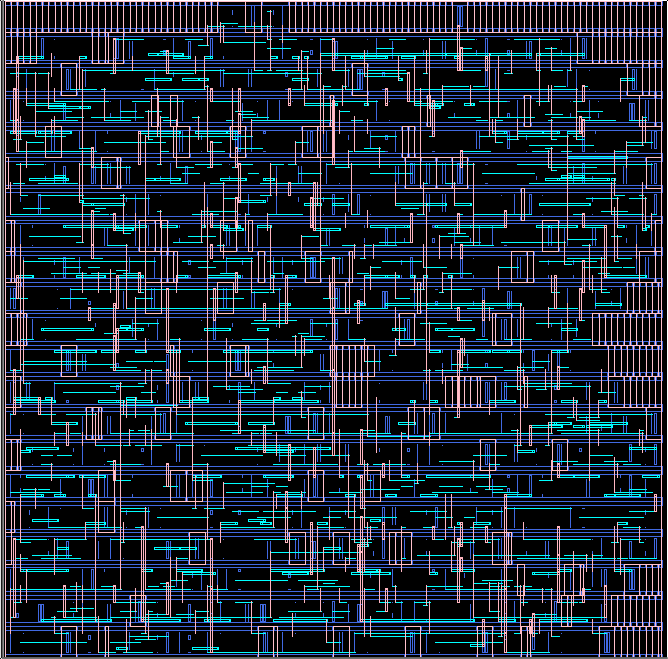
\includegraphics[width = 7cm]{pic/standard2.png}
\end{center}
\caption{Circuit glue logique avec 10\% de marge de surface.}
%\label{fig 4.}
\end{figure}

Concernant la partie chemin de données, nous n'avons pas réussi à faire le placement routage avec cgt, le programme segfault tout le temps sauf quand nous plaçons les cellules explicitement dans le code python ;  voici une partie du code python qui fait le placement:

\begin{python}
def Layout (self):
		Place ( self.mux, NOSYM, XY(0,0) )
		#PlaceLeft (self.mux, NOSYM)
		PlaceRight (self.accu, NOSYM)
		PlaceRight (self.adder, NOSYM)
		PlaceRight (self.buff, NOSYM)	
		self.View()
		return	
\end{python}

\begin{figure}
\begin{center}
  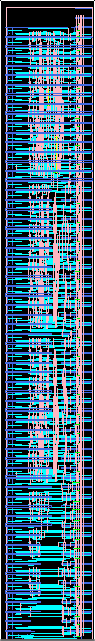
\includegraphics[width = 2cm]{pic/datapath.png}
\end{center}
\caption{Circuit chemin de données.}
%\label{fig 4.}
\end{figure}
\newpage
\section{TP3: Dessin de cellule}
\subsection*{}
Dans ce TP nous avons pu dessiner avec l'outil \textbf{Graal} le schéma de la cellule NAND, en se basant bien évidement sur ce que nous avons compris du cours et les démarches à suivre décrites dans le TP. Pour plus d’aide, nous nous sommes basés sur le schéma de la cellule NOR qui est disponible et que nous avons étudié en M1 dans l'UE VLSI1. Voici le layout final de la cellule:

\begin{figure}
\begin{center}
  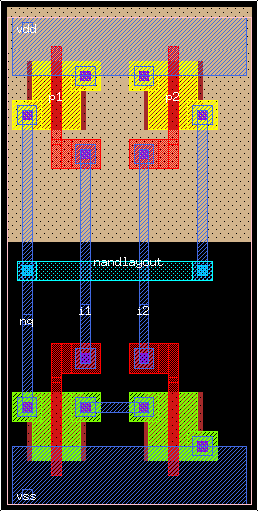
\includegraphics[width = 8cm]{pic/nand.png}
\end{center}
%\caption{Le chemin critique.}
%\label{fig 4.}
\end{figure}

Le makefile fournit permet d'extraire la netlist au format al à partir du format ap. il faut aussi noter que ce type d'extraction est une extraction au niveau transistor avec l'option -t\\
L’outil yagle permet d'extraire la description comportementale en VHDL à partir de la netlist .al.\\
Nous avons décrit en vhdl le comportement du nand dans le fichier nand.vbe, puis avec proof nous avons vérifié l'équivalence de notre description avec celle extraite avec yagle. Le comportement est le même sauf que la description est légèrement différente: \\
nand.vbe : s <= i0 nand i1;\\
nand\_yagle.vbe :  s <= not(i0) or not(i1);\\
Ceci est équivalent selon les règles de l'algèbre de Bool.\\
\end{document}
